\chapter{The Articulated Body Algorithm}
\label{ch:articulated_body_algorithm}
\label{laymans:context_box}

A torque at the wrist does not accelerate only the hand. The resulting joint accelerations depend on the configuration and inertia of the entire connected mechanism, the other applied torques, and its constraints. The articulated body algorithm (ABA) computes this coupled response efficiently for a rigid-body tree. Its value for golf is that it makes the mechanics calculable. It does not, by itself, identify a player's intention, solve ground contact, or determine which intervention improves club delivery.

\section{Historical Context: Recursive Forward Dynamics}
\label{sec:aba_history}

Featherstone's articulated-body formulation is a foundational recursive method for forward dynamics \cite{Featherstone1983,featherstone1987}. It exploits the tree structure of interconnected rigid bodies, eliminating one joint acceleration at a time and then recovering all accelerations. For a bounded number of degrees of freedom per joint, the unconstrained calculation takes work proportional to the number of bodies. This is an algorithmic statement, not a measured wall-clock time or a guarantee of accuracy for a chosen anatomical model.

Many useful dynamics calculations instead assemble the generalized mass matrix and solve a linear system. Neither method requires an explicit numerical matrix inverse. The right choice depends on the model, the quantities required, repeated right-hand sides, constraints and implementation. A fast solver cannot compensate for an incorrect inertia, omitted joint torque or unrealistic contact assumption.


\begingroup
\renewcommand*{\theHfigure}{aba.\arabic{figure}}
\begin{figure}[htbp]
\centering
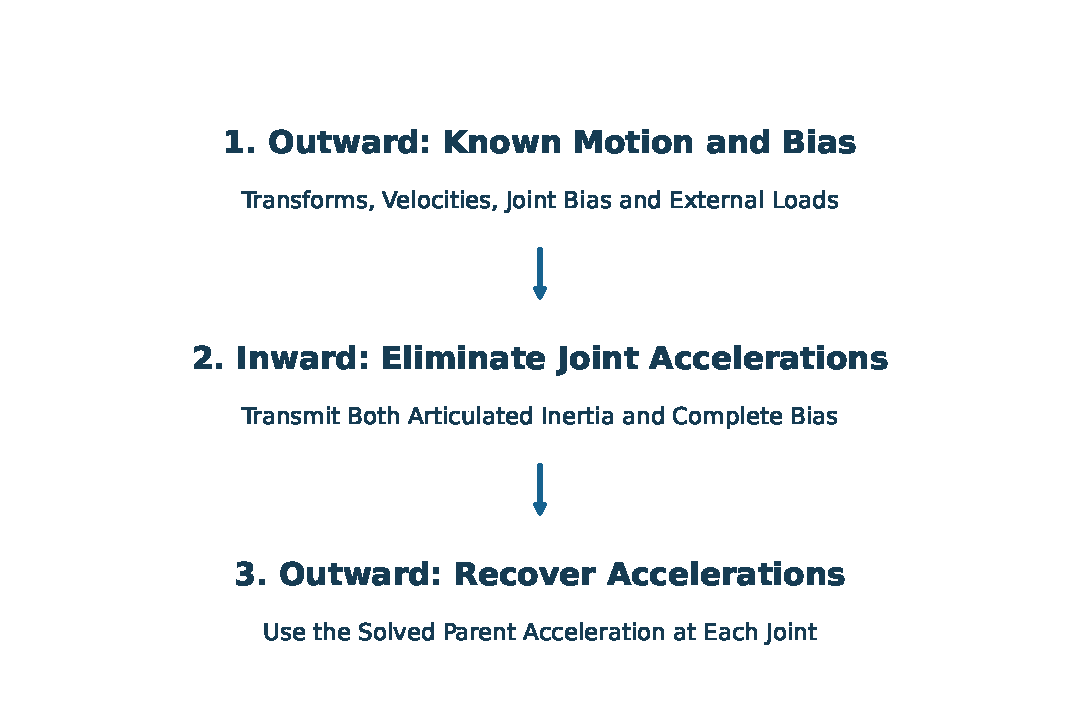
\includegraphics[width=0.92\linewidth]{../figures/articulated_body_passes.pdf}
\caption{Three Passes Through a Rigid-Body Tree: Compute Known Motion and Bias, Eliminate Joint Accelerations Inward, Then Recover Accelerations Outward.}
\label{fig:aba_passes}
\end{figure}
\endgroup


\section{The Forward Dynamics Problem}
\label{sec:forward_dynamics_problem}

\subsection{Problem Formulation}
\label{subsec:fd_formulation}

For a fixed-base mechanism with independent scalar joint coordinates, write
\begin{equation}
 M(q)\ddot q+h(q,\dot q)=\tau+Q_{\mathrm{ext}}.
\end{equation}
Here $M$ is the generalized inertia, $h$ contains velocity-dependent and gravitational terms, $\tau$ is the applied generalized joint force, and $Q_{\mathrm{ext}}$ represents other known external wrenches after projection into joint coordinates. A revolute joint's generalized force is a torque; a prismatic joint's is a force. All terms must use the same coordinate convention. Positive-definite $M$ gives a unique acceleration for these specified loads. It does not imply that the motion is dynamically stable.

Forward dynamics predicts acceleration from the state and loads. Inverse dynamics computes the generalized loads required by a prescribed acceleration. With contact or closed loops, one must additionally specify or solve for constraint reactions. With muscles, activation, force--length--velocity behavior and moment arms determine which joint torques can actually occur. Treating $\tau$ as a known input is a mechanical calculation, not a complete physiological model.

\subsection{What the Complexity Comparison Means}
\label{subsec:why_not_invert}

A generic dense positive-definite solve uses an $O(N^3)$ factorization followed by $O(N^2)$ work per right-hand side. That does not make a thirty-joint calculation impossible. Constants, hardware, numerical libraries, sparsity and reuse matter. Conversely, $O(N)$ does not imply that every implementation meets a particular control deadline. An operation count of $10^3$ at an assumed $10^9$ operations per second would correspond to one microsecond, not one nanosecond; real processors do not convert every mathematical operation into one clock cycle.

ABA avoids constructing the complete mass matrix when the immediate requirement is a tree acceleration solve. Collision detection, constraint solving, muscle dynamics, flexible shafts, integration and output derivatives are additional work. Their cost must not be hidden inside a claim that the whole golf simulation is linear-time.

\section{Articulated Inertia: The Key Insight}
\label{sec:articulated_inertia}

\subsection{A Free Hinge Changes the Apparent Load}
\label{subsec:inertia_intuition}

Imagine accelerating the proximal end of two connected links. If the hinge is locked, both links must satisfy that extra kinematic restriction. If it is free and its torque is specified, the distal link can accelerate relative to the proximal link. These two experiments generally produce different proximal reactions. Articulated inertia describes the second experiment after the distal joint accelerations have been eliminated. Composite rigid-body inertia describes the locked collection used in a different calculation.

This distinction matters when discussing a wrist release. A freely moving wrist, a commanded joint torque, a stiff feedback controller and a mechanically locked joint are different boundary conditions. They should not be represented by exchanging descriptive words while leaving the equations unchanged. The inertia appearing in ABA is an instantaneous mechanical response at a specified configuration and specified joint-force model; it is not a frequency-dependent closed-loop impedance.

\subsection{Mathematical Definition and Frames}
\label{subsec:articulated_inertia_math}

Use angular-first spatial motion $v_i=(\omega_i,v_{O_i})$ and moment-first spatial force $f_i=(n_{O_i},F_i)$, expressed in body frame $i$. Their pairing $f_i^T v_i$ is power. Let $X_i$ map motion coordinates from parent $p(i)$ into child $i$ for the same physical motion. Consequently a child wrench contributes $X_i^T f_i$ to its parent, and a child inertia contributes $X_i^T I_i X_i$. The transpose direction follows power invariance, not a visual resemblance between matrices.

After eliminating all joints strictly below body $i$, its subtree obeys
\begin{equation}
 f_i^A=I_i^A a_i+p_i^A.
 \label{eq:articulated_inertia}
\end{equation}
The unknown wrench $f_i^A$ is the wrench applied to that subtree through its proximal connection. The subtree bias $p_i^A$ includes known velocity terms, external loads and the effects of specified descendant torques. It is not merely friction or a force ``dragging'' the link. $I_i^A$ depends on geometry and inertias, and on any included ideal armature terms; it is generally not the spatial inertia of one rigid body.

The scalar joint direction $S_i$ maps $\dot q_i$ to relative spatial motion. It is a six-component motion vector, not an adjoint transformation. The derivation below assumes a constant subspace in the chosen joint/body frame, as for a standard one-degree-of-freedom revolute, prismatic or helical joint. General joint models need their own kinematic bias terms.

\section{Derivation From First Principles}
\label{sec:aba_derivation}

\subsection{Eliminating One Joint Acceleration}
\label{subsec:constraint_derivation}

At a fixed state, the kinematic acceleration relation is
\begin{equation}
 a_i=X_i a_{p(i)}+c_i+S_i\ddot q_i.
\end{equation}
Write $\bar a_i=X_i a_{p(i)}+c_i$. The unknown parent acceleration is kept separate from the known bias $c_i$. An ideal scalar joint satisfies $\tau_i=S_i^T f_i^A$. Substitute the subtree wrench relation to obtain
\begin{equation}
 \tau_i=S_i^T I_i^A\bar a_i+S_i^T I_i^A S_i\ddot q_i+S_i^T p_i^A.
\end{equation}
Define
\begin{equation}
 U_i=I_i^A S_i,\qquad d_i=S_i^T U_i,\qquad
 u_i=\tau_i-S_i^T p_i^A.
\end{equation}
Symmetry of $I_i^A$ then gives
\begin{equation}
 \ddot q_i=\frac{u_i-U_i^T\bar a_i}{d_i}.
\end{equation}
The scalar $u_i$ is a residual joint effort, not a six-dimensional wrench. For a physically nondegenerate model $d_i>0$. Dividing by a small or nonpositive value without investigating the model is not a stability remedy.

Substituting this acceleration back into the wrench relation gives
\begin{equation}
 f_i^A=I_i^a X_i a_{p(i)}+p_i^a,
 \qquad I_i^a=I_i^A-\frac{U_iU_i^T}{d_i},
\end{equation}
\begin{equation}
 p_i^a=p_i^A+I_i^a c_i+\frac{U_i u_i}{d_i}.
\end{equation}
Both terms are essential. The remainder $I_i^a$ represents the load transmitted after joint $i$ is allowed to accelerate under its specified torque. The transmitted bias includes the joint's torque effect even when velocities vanish. Dropping that term would prevent a distal applied torque from correctly influencing the proximal acceleration.

For positive-definite $I_i^A$, set $z=(I_i^A)^{1/2}S_i$. Then
\begin{equation}
 I_i^a=(I_i^A)^{1/2}
 \left(I-\frac{zz^T}{z^Tz}\right)(I_i^A)^{1/2}\succeq0,
 \qquad I_i^aS_i=0.
\end{equation}
The projection occurs in these inertia-weighted coordinates. It is not a Euclidean projection that says only motion along the joint contributes to the parent load. Rather, one freely accelerating direction has been eliminated. This is a Schur complement, the same algebraic operation used in block Gaussian elimination.

\section{The Articulated Body Algorithm: Three Passes}
\label{sec:aba_three_passes}

Number bodies so that parents precede children. The base is body $0$, and each nonbase body has one incoming joint. Known external wrenches must be expressed about and in the same frame as each body's inertia. Here gravity is included through a fictitious base acceleration, so it must not also be included as a body external load.

\subsection{Pass 1: Outward Velocity and Bias Calculation}
\label{subsec:pass1_outward}

\subsubsection{Spatial Velocity Propagation}
\label{subsubsec:velocity_propagation}

Start with $v_0=0$ for a fixed base. For each body in outward order,
\begin{equation}
 v_i^J=S_i\dot q_i,\qquad v_i=X_i v_{p(i)}+v_i^J.
\end{equation}
The transformed parent velocity already carries the effect of the parent origin's offset. Adding untransformed six-vectors would mix different physical reference points as well as orientations.

\subsubsection{Coriolis Acceleration and Bias Wrench}
\label{subsubsec:bias_force}

For angular-first $v=(\omega,v_O)$, define
\begin{equation}
 v\times=
 \begin{bmatrix}[\omega]_\times&0\\{[v_O]}_\times&[\omega]_\times\end{bmatrix},
 \qquad v\times^*=-(v\times)^T.
\end{equation}
The cross operator acting on motion differs from its dual acting on momentum or force. Initialize
\begin{equation}
 c_i=v_i\times v_i^J,\qquad I_i^A=I_i,\qquad
 p_i^A=v_i\times^*(I_i v_i)-f_i^{\mathrm{ext}}.
\end{equation}
For a more general joint, add its joint-specific acceleration bias to $c_i$. The Newton--Euler velocity wrench contains gyroscopic and centrifugal effects; it cannot be replaced by an arbitrary scalar multiple of angular speed. The external wrench is subtracted here because the unknown proximal wrench supplies only the part not already supplied externally.

\subsection{Pass 2: Inward Subtree Elimination}
\label{subsec:pass2_inward}

\subsubsection{Leaf Boundary Condition}
\label{subsubsec:leaf_inertia}

A leaf starts with its own rigid inertia and the bias just calculated. It has no child contribution. Process the bodies in reverse order so that all children have already contributed before their parent is eliminated.

\subsubsection{Recursive Inertia Update}
\label{subsubsec:inertia_recursion}

Compute $U_i,d_i,u_i,I_i^a,p_i^a$ from the one-joint derivation and accumulate
\begin{equation}
 I_{p(i)}^A\mathrel{+}=X_i^T I_i^a X_i.
 \label{eq:aba_inertia_recursion}
\end{equation}
The update adds every child's contribution. A branching tree is handled by summation, not by assuming one child or by overwriting an earlier contribution. Preserve $U_i,d_i,u_i$ for the final outward pass.

\subsubsection{Required Bias Propagation}
\label{subsubsec:bias_propagation}

The matching update is
\begin{equation}
 p_{p(i)}^A\mathrel{+}=X_i^T
 \left(p_i^A+I_i^a c_i+U_i u_i/d_i\right).
\end{equation}
This update is part of ABA, not an optional refinement. Inertia alone cannot describe a subtree's reaction at nonzero velocity or under a nonzero descendant torque. A static distal torque already changes the force balance transmitted proximally.

\subsection{Pass 3: Outward Acceleration Recovery}
\label{subsec:pass3_outward}

\subsubsection{Fixed-Base Acceleration and Gravity}
\label{subsubsec:base_acceleration}

For a stationary base in a uniform gravitational field $g$, set the algorithmic base acceleration to $a_0=(0,-g)$. Alternatively, use the physical zero base acceleration and supply gravity as external body forces consistently. Do not use both conventions simultaneously. The fixed base has a reaction wrench, generally nonzero, that can be recovered by inverse dynamics once the accelerations are known.

Spatial acceleration is also not simply a stack of ordinary angular and origin linear accelerations. In body coordinates its linear part is the ordinary origin acceleration minus $\omega_i\times v_{O_i}$, before accounting for the fictitious gravity convention. Comparing these arrays with accelerometer data therefore requires restoring the physical gravity/reference convention and the sensor's offset.

\subsubsection{Joint Acceleration Recovery}
\label{subsubsec:joint_acceleration}

For each body in outward order, compute
\begin{equation}
 \bar a_i=X_i a_{p(i)}+c_i,\qquad
 \ddot q_i=(u_i-U_i^T\bar a_i)/d_i,\qquad
 a_i=\bar a_i+S_i\ddot q_i.
 \label{eq:aba_joint_acceleration}
\end{equation}
No trigonometric approximation has been introduced by this elimination. It solves the stated rigid-body equations up to arithmetic error. Its agreement with an independent formulation checks the implementation, while experimental agreement checks the physical model. Those are separate questions.

\section{Why the Tree Calculation Is Linear-Time}
\label{sec:aba_complexity}

Each body requires a bounded number of operations on six-vectors and $6\times6$ matrices. Each edge transmits one inertia and one bias contribution. The three traversals therefore use $O(N)$ arithmetic and $O(N)$ storage for scalar joints. A joint with several degrees of freedom replaces $d_i$ by the block $S_i^T I_i^A S_i$ and requires a small linear solve. The linear-in-body-count statement assumes that block size is bounded.

Allocation and data structures also matter. Preallocated arrays or append-only lists followed by reverse traversal preserve the intended scaling. Repeated insertion at the front of a growing list can add quadratic data movement. Computing a complete dense derivative matrix, detecting contacts or solving a large contact system is not covered by the three-pass count.

\section{Floating Base: A Six-Degree-of-Freedom Root}
\label{sec:floating_base}
\index{floating-base dynamics}

\subsection{The Root Articulated Solve}
\label{subsec:floating_base_aba}

For a freely moving base, its acceleration is unknown. Initialize the base's own inertia and bias, include its known external wrench, and accumulate all child contributions. With the same fictitious-gravity convention and no unknown root constraint wrench,
\begin{equation}
 I_0^A a_0+p_0^A=0,\qquad a_0=-(I_0^A)^{-1}p_0^A.
\end{equation}
Implement this expression as a $6\times6$ solve. The matrix is the entire articulated subtree's inertia at the current configuration, not the isolated base's constant rigid inertia. Its factorization can be reused only while the quantities on which it depends remain unchanged. The remaining outward acceleration recovery is the same as before.

\subsection{Contact Does Not Automatically Fix the Base}
\label{subsec:contact_constraints}

A foot touching the ground may impose one normal constraint, several sticking constraints, or a finite contact-patch wrench model. It is not automatically a six-degree-of-freedom weld. A no-slip constraint is valid only while the required reaction satisfies the admitted friction and unilateral conditions. If the contact wrench is unknown, the root solve and contact equations must be resolved together; one cannot first assume an arbitrary base acceleration and then declare the resulting contact physically feasible.

\section{Floating-Base Humanoids and Momentum}
\label{sec:floating_base_humanoid}
\index{humanoid robot!dynamics}

\subsection{Configuration Coordinates and Generalized Velocity}
\label{subsec:virtual_joint}
\index{virtual joint}

A humanoid model may use a position and unit quaternion for the pelvis, together with joint coordinates. The quaternion has four stored components but only three rotational degrees of freedom. Write the state kinematics as $\dot q=N(q)\nu$, and dynamics in the generalized velocity $\nu$. In general $\nu\ne\dot q$. A six-dimensional root joint is a local motion description, not a requirement to use three globally nonsingular orientation angles; no such global three-angle chart exists.

\subsection{Root Equation With a Known Applied Wrench}
\label{subsec:base_acceleration}
\index{articulated inertia!floating base}

If a known additional root wrench $w_0$ is kept outside the bias convention, the root relation is
\begin{equation}
 I_0^A a_0=w_0-p_0^A.
 \label{eq:floating_base_accel}
\end{equation}
Count a wrench exactly once. An unknown ground reaction belongs to the constraint calculation, while a measured ground wrench can be supplied as known data within its measurement uncertainty. These choices answer different forward or inverse questions.

\subsection{Centroidal Momentum and Whole-Body Dynamics}
\label{subsec:centroidal_momentum}
\index{centroidal momentum}

Keep the angular-first ordering and define momentum about the total center of mass $c$:
\begin{equation}
 h_G=\begin{bmatrix}k_c\\p\end{bmatrix}=A_G(q)\nu,\qquad
 \dot h_G=
 \begin{bmatrix}
 \sum_j((r_j-c)\times F_j+n_j)\\
 m_{\mathrm{tot}}g+\sum_j F_j
 \end{bmatrix}.
 \label{eq:centroidal_momentum}
\end{equation}
The sums contain nongravitational external forces and couples. Uniform gravity has zero resultant moment about the total COM. Internal joint forces and torques cancel in the whole-system balance, but joint motion redistributes momentum among segments and changes $A_G$, the COM and contact moment arms. ``Internal torques cancel'' does not mean configuration is irrelevant.

For a golfer--club system, hand--club wrenches are internal only if both hands and the club are included in the system boundary. Ground reactions remain external. After ball contact, the ball must either be included or represented through an external interaction. This bookkeeping is necessary before attributing a rise in club momentum to any particular segment or source of work.

\section{Joint Friction and Motor Inertia}
\label{sec:friction_motor_inertia}

\subsection{Viscous Joint Friction}
\label{subsec:joint_friction}

For an ideal viscous coefficient $b_i\ge0$, use $\tau_i^{\mathrm{eff}}=\tau_i^{\mathrm{act}}-b_i\dot q_i$ in the joint elimination. The associated power is $-b_i\dot q_i^2\le0$. The induced acceleration is coupled through the dynamics; subtracting $b_i\dot q_i$ directly from a computed acceleration has both the wrong units and the wrong mechanical effect. Dry friction at zero velocity requires a separate set-valued or regularized model, not an arbitrary choice of sign presented as a universal law.

\subsection{An Ideal Reflected Armature Model}
\label{subsec:motor_inertia}

If a transmission is modeled by an independent rotor kinetic energy $J_i(r_i\dot q_i)^2/2$, its reflected armature is $a_i^{\mathrm{rot}}=r_i^2J_i$. Under precisely that idealization, the joint equation includes $a_i^{\mathrm{rot}}\ddot q_i$, and the pivot becomes
\begin{equation}
 d_i=S_i^T I_i^A S_i+a_i^{\mathrm{rot}}.
\end{equation}
Use this pivot in the remainder, transmitted bias and acceleration recovery. The remainder no longer generally annihilates $S_i$. General rotor/body coupling, flexible transmissions and configuration-dependent gearing require a fuller kinetic model. Muscles are not rotary motors with a freely chosen reflected rotor inertia; their activation and force-generation dynamics must be modeled on their own terms.

\section{ABA and Composite Rigid-Body Methods}
\label{sec:aba_vs_crba}

The composite rigid-body algorithm (CRBA) constructs $M(q)$ from locked-subtree inertias. Its worst-case assembly cost is $O(N^2)$ for a scalar-joint tree. In a serial chain, distant joint velocities can contribute to the same body's kinetic energy, so the mass matrix is generally dense. A branched tree has an ancestor-dependent sparsity pattern, not a universally bounded bandwidth.

For one unconstrained right-hand side, ABA can avoid forming $M$. If an application already needs $M$ for constraints, identification or optimization, factorization may be useful. At fixed configuration, a dense factorization is reused at $O(N^2)$ per additional right-hand side; a suitably organized articulated factorization can apply the inverse in $O(N)$ per right-hand side. Constructing $R$ complete solutions still requires their output and load processing. No numeric runtime comparison follows from stating these asymptotic orders alone.

\section{Choosing Forward or Inverse Dynamics}
\label{sec:fd_id_decision}

\subsection{When the Acceleration Is Prescribed}
\label{subsec:use_id}

Use inverse dynamics to find the generalized force required by a specified motion and external-load model. In a measured swing, differentiation noise, inertial estimates and ground/contact measurements strongly affect this calculation. A net joint torque is not a unique decomposition into individual muscle forces. If external forces are unknown, kinematics alone may not determine all loads.

\subsection{When the Applied Loads Are Specified}
\label{subsec:use_fd}

Use forward dynamics to compare predicted accelerations or trajectories under explicit loading or control changes. Holding all other joint torques fixed while changing one torque gives a well-defined instantaneous intervention in the unconstrained model. Holding a feedback policy fixed over a new trajectory is a different experiment from replaying the original torque history. A claimed improvement in club delivery must state which experiment was performed and how ground, grip and muscle feasibility were maintained.

\section{Constraint Handling: Contact and Joint Limits}
\label{sec:constraints}

\subsection{Unilateral Contact}
\label{subsec:contact}

Let $\phi(q)$ be a signed normal gap: $\phi>0$ means separation and $\phi=0$ means touching. An ideal rigid contact requires $\phi\ge0$ and a compressive normal reaction $\lambda_n\ge0$. A separated contact does not supply a force merely because its unconstrained acceleration points toward the surface. A closing trajectory needs event detection or a consistent time-stepping scheme; sustained-contact acceleration equations do not describe an instantaneous impact.

\subsection{Joint Limits}
\label{subsec:joint_limits}

A hard lower or upper joint limit can be represented by a unilateral gap in configuration space, with its own reaction or impact rule. A soft limit instead supplies a specified force law. Abruptly clipping the angle after integration can violate momentum and inject or remove energy without a stated model. Anatomical range limits, passive tissue forces and active control are related but distinct phenomena.

\section{Connection to Gaussian Elimination}
\label{sec:gaussian_elimination_connection}

The one-joint derivation is block elimination of coupled wrench and acceleration equations. ABA performs this elimination on a spatial tree representation. It does not require the generalized mass matrix to be band diagonal. The Schur complement is exact for the stated algebra; its numerical evaluation still depends on scaling and conditioning. Very small inertias, inconsistent units, nonphysical mass parameters and cancellation can produce poor numerical results in a recursive or matrix formulation.

For example, partition a three-joint mass matrix into proximal coordinate $q_1$ and distal coordinates $q_d$. At zero velocity and gravity, with $\tau_d=0$,
\begin{equation}
 M_{\mathrm{eff}}=M_{11}-M_{1d}M_{dd}^{-1}M_{d1},\qquad
 \ddot q_1=\tau_1/M_{\mathrm{eff}}.
\end{equation}
With the distal joints locked instead, the corresponding coefficient is $M_{11}$. The difference expresses the mechanical effect of allowing relative motion, not evidence that a golfer should minimize effective inertia throughout the swing. Club orientation, feasible torque, shaft deformation and impact conditions impose additional objectives and restrictions.

\section{Worked Example: A Fully Specified Three-Link Arm}
\label{sec:worked_example_aba}

Consider three uniform solid cylinders of lengths $(0.4,0.3,0.25)$ m, masses $(2.0,1.2,0.6)$ kg and common radius $0.025$ m. Their local $x$ axes run along the links; all joints rotate about local $z$. Each body frame originates at its proximal joint. This is an ideal teaching mechanism, not measured anatomy or a fitted golf club. The finite radius gives physically consistent positive rotational inertias.

For each cylinder, $c_i=(L_i/2,0,0)$ and
\begin{equation}
 I_{C_i}=\operatorname{diag}
 \left(\frac{m_i r^2}{2},\frac{m_i(L_i^2+3r^2)}{12},
 \frac{m_i(L_i^2+3r^2)}{12}\right),
\end{equation}
\begin{equation}
 I_i=\begin{bmatrix}
 I_{C_i}+m_i[c_i]_\times[c_i]_\times^T&m_i[c_i]_\times\\
 m_i[c_i]_\times^T&m_i I_3
 \end{bmatrix}.
\end{equation}
The upper-left parallel-axis contribution is added. The off-diagonal blocks follow from the COM offset and must not be invented independently.

\subsection{Configuration and Loads}
\label{subsec:config_aba}

Use relative angles $q=(0.4,-0.7,0.2)$ rad, rates $\dot q=(0.8,-0.5,1.1)$ rad/s and actuator torques $\tau=(4,-1,0.3)$ N m. Gravity is $(0,-9.81,0)$ m/s$^2$. There are no other external wrenches, no damping and no armature in this particular calculation.

Let $E_i=R_z(q_i)^T$ reexpress parent-oriented components in child axes, and let $r_i=(L_{i-1},0,0)$ be the parent-frame joint offset, with $r_1=0$. Then
\begin{equation}
 X_i=\begin{bmatrix}E_i&0\\-E_i[r_i]_\times&E_i\end{bmatrix},
 \qquad S_i=(0,0,1,0,0,0)^T.
\end{equation}
The joint angles therefore enter every transform. The relative angles are not interchangeable with the links' absolute orientations, which are $(0.4,-0.3,-0.1)$ rad.

\subsection{Pass 1: Velocities and Bias}
\label{subsec:pass1_example}

All out-of-plane components vanish. Listing each spatial velocity as the planar triple $(\omega_z,v_x,v_y)$, the outward recursion gives
\begin{equation}
 \begin{aligned}
 v_1&=(0.8,0,0),\\
 v_2&=(0.3,-0.206149660,0.244749500),\\
 v_3&=(1.4,-0.135535933,0.369032412).
 \end{aligned}
\end{equation}
The angular components sum relative rates, while the linear components also require rotations and joint-origin offsets. Form $c_i=v_i\times S_i\dot q_i$ and the initial $p_i^A=v_i\times^*I_i v_i$ from these complete velocities. There is no arbitrary bias-force estimate.

\subsection{Pass 2: Articulated Inertias and Residual Efforts}
\label{subsec:pass2_example}

The planar subblocks of the articulated inertias, before eliminating each body's own joint, are approximately
\begin{equation}
 I_3^A\big|_{zxy}=
 \begin{bmatrix}0.012593750&0&0.075000000\\0&0.600000000&0\\0.075000000&0&0.600000000\end{bmatrix},
\end{equation}
\begin{equation}
 I_2^A\big|_{zxy}=
 \begin{bmatrix}0.051575604&0.026090063&0.231293680\\
 0.026090063&1.782370942&0.086966875\\
 0.231293680&0.086966875&1.370978934\end{bmatrix},
\end{equation}
\begin{equation}
 I_1^A\big|_{zxy}=
 \begin{bmatrix}0.260428859&-0.284953502&0.783624232\\
 -0.284953502&3.143841922&-0.712383755\\
 0.783624232&-0.712383755&2.959060579\end{bmatrix}.
\end{equation}
The rotational, mixed and translational entries carry different SI units. These subblocks are sufficient to display this planar example, but the implementation uses full six-dimensional quantities. The pivots and residual joint efforts are
\begin{equation}
 \begin{aligned}
 d&=(0.260428859,0.051575604,0.012593750),\\
 u&=(6.518800728,-1.799610488,0.314231273).
 \end{aligned}
\end{equation}
Gravity has not yet entered these residual efforts because it enters through the fictitious base acceleration in pass 3. The residuals differ from the supplied torques because the inward bias carries descendant loads and velocity effects.

\subsection{Pass 3 and an Independent Check}
\label{subsec:pass3_example}

Outward recovery gives, in rad/s$^2$,
\begin{equation}
 \ddot q=(2.023035078,-79.465503634,175.204404572).
\end{equation}
These large distal accelerations reflect the particular light-link model and loads. They are not plausible-muscle bounds or a prediction for a human swing. To check the result independently, form the Cartesian COM Jacobians $J_{C_i}$ and angular Jacobians $J_{\omega_i}$ from the link positions. Kinetic energy gives
\begin{equation}
 M=\sum_i\left(m_iJ_{C_i}^TJ_{C_i}+J_{\omega_i}^T I_{C_i}^{\mathrm{world}}J_{\omega_i}\right).
\end{equation}
For these planar coordinates, differentiating this mass matrix gives the Christoffel velocity terms, and differentiating gravitational potential gives the gravitational terms. The independent calculation produces
\begin{equation}
 M=\begin{bmatrix}
 0.814792916&0.283348998&0.060972725\\
 0.283348998&0.146884246&0.034645248\\
 0.060972725&0.034645248&0.012593750
 \end{bmatrix},
\end{equation}
\begin{equation}
 h=(14.185426211,4.029005575,0.723271650)^T.
\end{equation}
Solving $M\ddot q=\tau-h$ agrees with ABA. The displayed values are rounded; residual checks use full precision. Tests additionally check nonzero external wrenches, damping and armature, multiple configurations, branched prismatic motion and reexpression in different body frames. Agreement across these cases is stronger evidence than checking an example against a second transcription of the same inward recursion.

\section{Reproducible Python Example}
\label{sec:python_aba_example}

The repository implementation is split between the generic prepared-tree solver and a cylinder-chain model builder. It uses the existing checked spatial-inertia and cross-product functions. Its inputs are explicitly restricted to a fixed-base rigid tree with constant local scalar-joint subspaces. It does not silently treat a contact or a flexible link as such a joint. The following example runs from the repository root:

\begin{lstlisting}[language=Python,basicstyle=\ttfamily\small]
import numpy as np
from src.tools.articulated_chain_examples import cylinder_chain
from src.tools.articulated_body_examples import (
    DynamicsLoads, forward_dynamics, inverse_dynamics,
)

tree = cylinder_chain(
    np.array([0.4, 0.3, 0.25]),
    np.array([2.0, 1.2, 0.6]),
    np.array([0.4, -0.7, 0.2]),
    0.025,
)
loads = DynamicsLoads(
    velocity=np.array([0.8, -0.5, 1.1]),
    torque=np.array([4.0, -1.0, 0.3]),
)
result = forward_dynamics(tree, loads)
print(result.joint_acceleration)
print(result.pivot)
recovered = inverse_dynamics(
    tree, loads, result.joint_acceleration
)
np.testing.assert_allclose(recovered, loads.torque)
\end{lstlisting}

The diagnostic result exposes velocities, articulated inertias, biases, pivots and residual efforts for inspecting the derivation. Array shapes, finite loads, ordered parents and positive-definite body inertias are checked. Physical rigid-body inertia structure and valid rigid motion transforms remain modeling preconditions. The supplied cylinder builder constructs them from positive dimensions. Invalid or nonpositive articulated pivots raise an error; assigning zero acceleration would conceal a broken or degenerate model.

In NumPy, a one-dimensional vector's transpose is still one-dimensional. To form $U_iU_i^T$, call \texttt{np.outer} with the vector as both arguments. For a one-dimensional array, \texttt{U @ U.T} instead returns a scalar, which can silently broadcast into an incorrect matrix update.

\subsection{Connection to Simulation Frameworks}
\label{subsec:simulation_frameworks}

Different simulators use different combinations of recursive dynamics and constraint solvers. MuJoCo's documented computation path forms its mass matrix with CRB and uses sparse $L^TDL$ factorization and back-substitution \cite{MuJoCoComputationReview}. It must not be described as using ABA for every timestep. Pinocchio provides ABA and analytical dynamics derivatives, along with other algorithms \cite{PinocchioSoftwareReview}. These statements identify documented methods; they do not rank accuracy or runtime. A reproducible comparison must identify software versions, model parameters, contact and integration settings, hardware and the actual quantity timed.

\section{Contact Forces and Impact Dynamics}
\label{sec:contact_impact}

During smooth motion, a force changes acceleration. An ideal instantaneous impact changes velocity while configuration remains continuous. For a single frictionless contact with normal Jacobian $J_n$, closing velocity $v_n^-=J_n\nu^-<0$ and restitution coefficient $0\le e\le1$,
\begin{equation}
 M(\nu^+-\nu^-)=J_n^T\Lambda_n,\qquad
 J_n\nu^+=-eJ_n\nu^-,
\end{equation}
\begin{equation}
 \Lambda_n=-\frac{(1+e)J_n\nu^-}{J_nM^{-1}J_n^T}.
\end{equation}
Here $M$ and $J_n$ are evaluated at the impact configuration and the denominator is positive for a nonzero contact direction and positive-definite $M$. The resulting impulse is compressive. It has impulse units, unlike the sustained reaction force. Multiple simultaneous contacts, friction and restitution require a specified coupled impact law; independent application of this scalar formula need not be consistent.

Ball impact also involves ball spin, clubface geometry and material deformation. This scalar illustration does not replace a validated ball--club collision model. It explains why comparing only pre-impact accelerations cannot establish a post-impact delivery or ball-flight claim.

\section{Contact Dynamics and Complementarity}
\label{sec:contact_lcp}
\index{contact dynamics}

\subsection{Non-Penetration and Sustained Contact}
\label{subsec:complementarity}
\index{complementarity condition}
\index{Signorini conditions}

At a closed contact with zero normal velocity, define normal acceleration $a_n=J_n\dot\nu+\dot J_n\nu$. An ideal frictionless acceleration-level condition is
\begin{equation}
 a_n\ge0,\qquad\lambda_n\ge0,\qquad a_n\lambda_n=0.
 \label{eq:complementarity}
\end{equation}
The alternatives are separating acceleration with zero reaction, or a compressive reaction maintaining zero normal acceleration. These conditions apply to the specified closed, nonimpacting candidate contacts. They are not a universal replacement for the gap and velocity conditions along an arbitrary trajectory.

\subsection{Friction and Contact Wrenches}
\label{subsec:friction_cone}
\index{friction cone}
\index{Coulomb friction}

For a point contact, the Coulomb force cone is
\begin{equation}
 \|\lambda_t\|\le\mu\lambda_n,\qquad\lambda_n\ge0.
 \label{eq:coulomb_friction}
\end{equation}
This inequality bounds the tangential force but does not specify its value during sliding. A sliding law ordinarily also imposes opposition to slip or a maximum-dissipation condition. A finite foot patch can transmit moments subject to geometry and pressure restrictions; a three-dimensional force cone is not the complete admissible six-dimensional wrench set. Rigid frictional contact can exhibit nonuniqueness or inconsistency, so no simple cone equation should be advertised as solving all contact physics exactly.

\subsection{The Frictionless Acceleration LCP}
\label{subsec:lcp_formulation}
\index{linear complementarity problem}
\index{LCP|see {linear complementarity problem}}

For a chosen set of closed, zero-normal-velocity contacts, write
\begin{equation}
 M\dot\nu+h=\tau+J_n^T\lambda_n.
 \label{eq:constrained_dynamics}
\end{equation}
Let $a_{\mathrm{free}}=M^{-1}(\tau-h)$, $W=J_nM^{-1}J_n^T$ and $b=J_n a_{\mathrm{free}}+\dot J_n\nu$. Then
\begin{equation}
 a_n=W\lambda_n+b,\qquad
 0\le\lambda_n\perp a_n\ge0.
 \label{eq:lcp}
\end{equation}
The matrix $W$ is positive semidefinite. Redundant contact directions can make reaction forces nonunique even when the resulting acceleration is determined. Friction introduces additional modeling choices; this frictionless LCP is not the full frictional problem.

ABA can supply products with $M^{-1}$ for constructing or applying $W$. Each such product is a tree solve, but assembling and solving the contact problem has its own cost. The number and arrangement of contacts and the chosen numerical method matter. Soft-contact formulations, including MuJoCo's documented model, make different assumptions from exact rigid complementarity.

\subsection{Time-Stepping and Numerical Order}
\label{subsec:time_stepping}
\index{time-stepping methods}

A velocity step using an impulse $\Lambda$ may take the form
\begin{equation}
 M(q_k)(\nu_{k+1}-\nu_k)
 =\Delta t\,(\tau_k-h_k)+J(q_k)^T\Lambda.
 \label{eq:time_stepping}
\end{equation}
This frozen-coefficient expression is not, by itself, full implicit Euler. The contact law, evaluation points and configuration update define the method. Restitution and stabilization also affect the result.

The familiar velocity-first Euler update is first order. In canonical separable Hamiltonian coordinates the corresponding symplectic Euler method is symplectic; a velocity-first update for a configuration-dependent multibody mass matrix does not inherit that claim automatically. Velocity Verlet is second order for its appropriate position-force/separable setting. General velocity-dependent multibody dynamics and impacts require an integrator suited to those equations. Check convergence as the timestep decreases, constraint residuals and energy/momentum behavior under the stated force model. An accurate acceleration solve does not remove integration error.

\section{From Coupled Dynamics to a Golf-Swing Argument}

For smooth unconstrained motion at a fixed state, the immediate torque-to-acceleration sensitivity is $\delta\ddot q=M^{-1}\delta\tau$. With bilateral constraints $J\dot\nu+b_c=0$ and full-row-rank $J$, solving for the reaction gives the constrained acceleration sensitivity
\begin{equation}
 \delta\dot\nu=P_M\delta\tau,\qquad
 P_M=M^{-1}-M^{-1}J^T(JM^{-1}J^T)^{-1}JM^{-1}.
\end{equation}
The reaction changes when a torque changes. Holding the old contact force fixed would answer a different question and can violate the constraint. Both hands on a rigid club close a kinematic loop through the arms and torso; a cut-tree ABA calculation must restore that loop through constraints or an explicitly compliant grip model.

This instantaneous response is only one component of delivery. If $x$ includes configuration, velocity, muscle activation and any shaft states, an implemented policy produces a field $\dot x=F_\pi(x,t)$. For an additional input perturbation with local input derivative $B_\pi$, the finite-interval variational equation is
\begin{equation}
 \delta\dot x=D_xF_\pi\,\delta x+B_\pi\,\delta u.
\end{equation}
The state derivative includes the feedback policy's response to state changes. The club's selected output at a fixed time depends on the propagated state perturbation and the output derivative. At a state-triggered impact, event-time and reset sensitivities are also required. A torque change may improve one output while worsening face angle, path, contact location or robustness. Segment speed peaks alone do not identify which muscles caused those changes.

A strong swing analysis therefore states its system boundary, inertia and joint model, admitted ground/grip reactions, actuator policy, perturbation and delivery outcome. It checks mechanical consistency before drawing a coaching conclusion. Energy and momentum balances supply complementary checks: internal joint action can redistribute momentum and perform work, but a sequence of angular-speed maxima is neither an energy-flow measurement nor proof of a unique optimal release strategy.

\section{Differentiating the Dynamics}

For a smooth, nonsingular fixed model, differentiating $M\ddot q+h=\tau$ gives
\begin{equation}
 \delta\ddot q=M^{-1}
 \left(\delta\tau-\delta h-(\delta M)\ddot q\right).
\end{equation}
This identity clarifies the derivative target independently of a software implementation. Automatic differentiation can propagate derivatives through a correctly implemented smooth recursion. Analytical derivative algorithms provide another route. Neither produces exact real-number arithmetic or an automatic derivative through every switching contact event. Differentiating the integrated or hybrid map requires its additional chain rules and event assumptions.

The full dense Jacobian has quadratically many entries in the number of joints. A directional derivative or reverse-mode derivative of a scalar objective can have a different cost from materializing every entry. Benchmark the actual requested derivative and include contact, controller and integration work before asserting a learning or control rate.

\section{Chapter Summary}
\label{sec:ch10_summary}

ABA solves the specified rigid-tree forward problem through outward kinematics, inward elimination and outward recovery. The essential quantities are the articulated inertia and its complete bias, transformed through power-consistent frames. Articulating and locking a subtree are different mechanical experiments. Floating bases, actuator models, contact and impact require their own explicit assumptions. The independently checked example establishes computational consistency; applying the method to golf additionally requires a validated model and a clearly defined causal or predictive question.

\section{Further Reading and References}
\label{sec:ch10_further_reading}

Featherstone's original formulation and later treatment provide the recursive dynamics foundation \cite{Featherstone1983,featherstone1987}. His Spatial\_v2 documentation provides inspectable reference algorithms and coordinate-transform conventions \cite{FeatherstoneSpatialReview}. MuJoCo's computation documentation and Pinocchio's software description document distinct implementation choices \cite{MuJoCoComputationReview,PinocchioSoftwareReview}. The calculations here are derived explicitly and checked independently; consulting these sources does not substitute for stating the model and experiment used in a golf argument.

\section{Exercises}
\label{sec:ch10_exercises}

\begin{enumerate}
\item \textbf{Complexity Analysis:} Count the bounded-size operations in all three passes for scalar joints. Identify the assumptions needed for $O(N)$ work and storage. Explain why constructing all dense acceleration derivatives or solving contact is additional work.
\item \textbf{Articulated and Composite Inertia:} Use three cylinders with $m_i=1$ kg, $L_i=1$ m, radius $0.05$ m and $q=(0.2,-0.4,0.3)$ rad. Calculate every articulated inertia with the distal joints free, and every composite inertia with them locked. Explain the difference without treating a singular point-mass inertia as a generic rigid body.
\item \textbf{Motor Inertia:} Add $0.04$ kg m$^2$ of ideal armature to joint 1 of the worked example. Recalculate all accelerations. Derive the sensitivity using the rank-one change in $M$, and explain why distal accelerations can change even though their own armatures are unchanged.
\item \textbf{Floating Base:} Describe the extra root quantities and solve for a thirty-joint floating-base mechanism. Separate its additional bounded-size root work from the effects of adding contact constraints. Do not infer an exact runtime ratio from the degree-of-freedom count.
\item \textbf{Repeated Right-Hand Sides:} At fixed $q$ and $\dot q$, compare reuse of a dense mass factorization and an articulated factorization for one hundred torque vectors. State preparation, per-solve and storage costs separately. Explain which quantities must be refreshed if $\dot q$ or $q$ changes.
\item \textbf{Bias Verification:} Restrict the worked model to its first two links at $q=(0.4,-0.7)$ and $\dot q=(0.8,-0.5)$. Calculate velocity forces from the spatial recursion and from Christoffel terms of the Cartesian kinetic-energy mass matrix. Compare gravity separately to avoid confusing force conventions.
\item \textbf{Singular Pivots:} Prove $d_i>0$ for a nonzero $S_i$ and positive-definite $I_i^A$ without armature. Explain how massless idealizations, degenerate coordinates or nonphysical parameters can defeat this condition. Why is replacing a zero pivot by zero acceleration not a valid solution?
\item \textbf{Joint Damping:} Add coefficients $(0.2,0.1,0.03)$ N m s/rad to the worked example. Verify $\tau^{\mathrm{eff}}=\tau-B\dot q$ before the solve and that the damping power is nonpositive. Compare against the incorrect post-solve acceleration subtraction.
\item \textbf{Gravity Simulation:} Construct four identical cylinders of length $0.3$ m, mass $1$ kg and radius $0.025$ m, initially at $q=(0.4,-0.2,0.3,-0.1)$ with zero rates. Simulate gravity-only motion with a fixed proximal base. State the integrator, refine the timestep, and monitor total mechanical energy; a fixed-base pendulum chain is not whole-body ballistic free fall.
\item \textbf{Contact Impulse:} For the first two worked links at $q=(0.4,-0.7)$, define a horizontal surface through the distal endpoint and use $\dot q=(-0.8,-0.5)$. Form the endpoint's upward normal Jacobian. Compute the single frictionless impulse for $e=0$ and verify the post-impact normal velocity and nonnegative impulse. Distinguish this velocity jump from subsequent sustained-contact acceleration.
\item \textbf{Integration Order:} Compare a first-order velocity-first method with a suitable second-order method on a smooth problem. Verify observed convergence against a refined reference. Explain when the words symplectic and Verlet apply, and why an impact can invalidate a smooth-step order argument.
\item \textbf{Matrix Formulation:} Build a specified ten-link cylinder chain and compare ABA with a positive-definite linear solve using its assembled $M$ and bias. Report residuals and conditioning; do not explicitly invert $M$ merely to apply it to one vector.
\item \textbf{Floating-Base Reactions:} For a specified humanoid model, choose either a point-foot or a finite-patch contact model. Write the root and contact equations together. State the rank, friction and unilateral conditions required for the computed reaction, and explain what measured contact data would remove from the unknowns.
\item \textbf{Redundancy:} Choose a task Jacobian $J$ for the worked model. Examine the map $JM^{-1}\delta\tau$ and construct a torque perturbation with zero immediate task acceleration when such a null space exists. Explain why that does not imply zero state change or unchanged delivery at a later time.
\item \textbf{Constrained Projection:} Let $M\succ0$ and full-row-rank $J$ be fixed, and require $Ja+b_c=0$. Minimize $(a-a_{\mathrm{free}})^TM(a-a_{\mathrm{free}})/2$ under that constraint. Derive $a=a_{\mathrm{free}}-M^{-1}J^T(JM^{-1}J^T)^{-1}(Ja_{\mathrm{free}}+b_c)$. Explain why this is a mass-weighted closest acceleration, not an arbitrary Euclidean minimum-norm forward solution, and discuss redundant constraints separately.
\end{enumerate}
